\documentclass[12pt,a4paper]{article}
\usepackage[utf8]{inputenc}
\usepackage{amsmath}
\usepackage{amsfonts}
\usepackage{amssymb}
\usepackage{graphicx}
\usepackage[left=2cm,right=2cm,top=2cm,bottom=2cm]{geometry}
\author{leonardo}
\begin{document}
\chapter{¿Que es un amplificador operacional?}
\begin{center}
•

Un amplificador operacional, a menudo conocido opamp por sus siglas en inglés (operational amplifier) es un dispositivo amplificador electrónico de alta ganancia acoplado en corriente continua que tiene dos entradas y una salida. En esta configuración, la salida del dispositivo es, generalmente, de cientos de miles de veces mayor que la diferencia de potencial entre sus entradas.
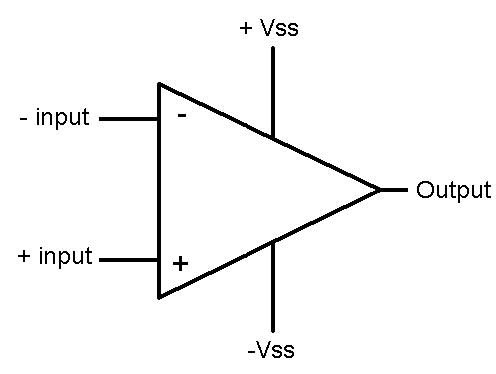
\includegraphics[width=7cm]{ampli.jpg} 
\end{center}

\begin{flushleft}
 Pasa altas: Solo dejan pasar las frecuencias que están por debajo de una determinada frecuencia, la cual es un capacitor arriba y una rsitencia 
 \end{flushleft} 
\begin{flushleft}
Pasa bajas:olo dejan pasar aquellas frecuencias que sean mayores de determinada frecuencia, la cual es la resistencia arriba y despues el capacitor
\end{flushleft}
\begin{flushleft}
Pasa banda:olo dejan pasar aquellas frecuencias que sean mayores de determinada frecuencia.
\end{flushleft}
\chapter{Tipos de arreglos }

\begin{flushleft}
Amplificador inversor:La configuración básica del AO. El amplificador inversor. En este circuito, la entrada (+) está a masa, y la señal se aplica a la entrada (-) a través de R1, con realimentación desde la salida a través de R2.
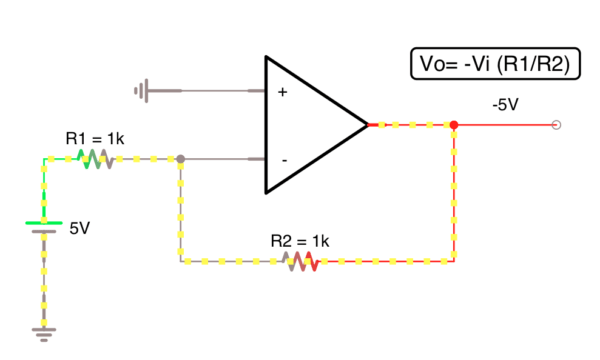
\includegraphics[wedth=7cm]{Inversor.png} 

\end{flushleft}
\begin{flushleft}
Amplificadres no inversor:En este circuito, la tensión Vi se aplica a la entrada (+), y una fracción de la señal de salida, Vo, se aplica a la entrada (-) a través del divisor de tensión R1 – R2. Puesto que, no fluye corriente de entrada en ningún terminal de entrada, y ya que Vd = 0, la tensión en R1 será igual a Vi.
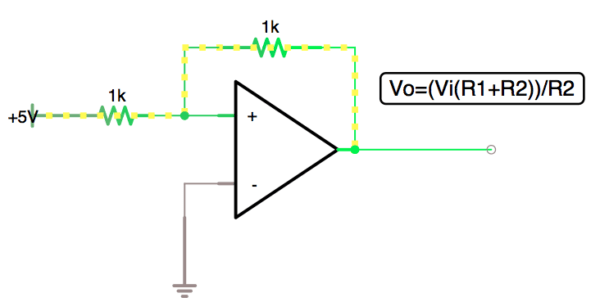
\includegraphics[wedth=7cm]{no-inversor.png} 
\end{flushleft}
\begin{flushleft}
Amplificador diferencial:Una tercera configuración del AO conocida como el amplificador diferencial, es una combinación de las dos configuraciones anteriores. Aunque está basado en los otros dos circuitos, el amplificador diferencial tiene características únicas. Este circuito, tiene aplicadas señales en ambos terminales de entrada, y utiliza la amplificación diferencial natural del amplificador operacional.

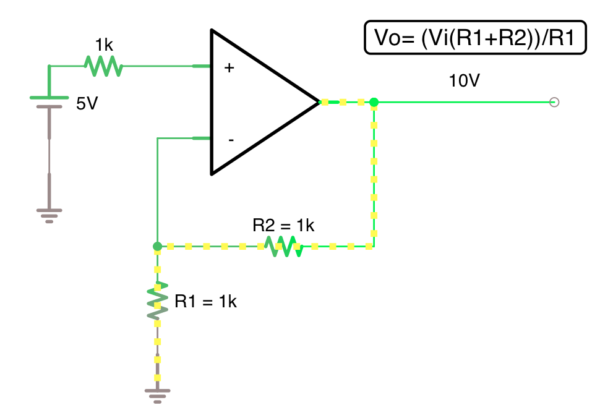
\includegraphics[wedth=7cm]{3.png} 
\end{flushleft}
\begin{flushleft}
Sumador inverso:Utilizando la característica de tierra virtual en el nudo suma (-) del amplificador inversor, se obtiene una útil modificación, el sumador inversor
En este circuito, como en el amplificador inversor, la tensión V(+) está conectada a masa, por lo que la tensión V(-) estará a una masa virtual, y como la impedancia de entrada es infinita toda la corriente I1 circulará a través de RF y la llamaremos I2. Lo que ocurre en este caso es que la corriente I1 es la suma algebraica de las corrientes proporcionadas por V1, V2 y V3.
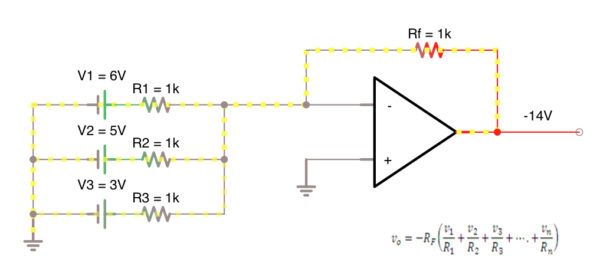
\includegraphics[scale=1]{sumainver.jpg} 
\end{flushleft}
\begin{flushleft}
El integrador:Se ha visto que ambas configuraciones básicas del AO actúan para mantener constantemente la corriente de realimentación, IF igual a IIN.
Una modificación del amplificador inversor, el integrador, se aprovecha de esta característica. Se aplica una tensión de entrada VIN, a RG, lo que da lugar a una corriente IIN.
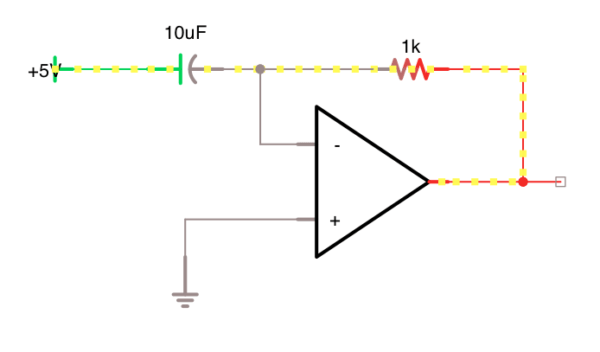
\includegraphics[wedth=7cm]{6.png} 
\end{flushleft}
\begin{flushleft}
Elseguidor de tension:Una modificación especial del amplificador no inversor es la etapa de ganancia.
En este circuito, la resistencia de entrada se ha incrementado hasta infinito, y RF es cero, y la realimentación es del 100%. V0 es entonces exactamente igual a Vi, dado que Es = 0. El circuito se conoce como “seguidor de emisor” puesto que la salida es una réplica en fase con ganancia unidad de la tensión de entrada. La impedancia de entrada de esta etapa es también infinita
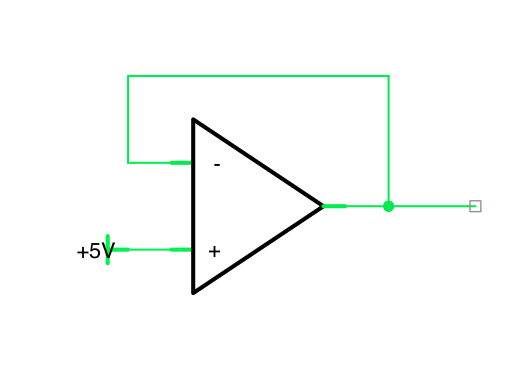
\includegraphics[wedth=7cm]{7.png} 
\end{flushleft}
\chapter{¿Cual es la diferencia entre la clase  a y la b?}
\begin{flushleft}
•un amplificador de potencia funciona en clase A cuando la tensión de polarización y la amplitud máxima de la señal de entrada poseen valores tales que hacen que la corriente de salida circule durante todo el período de la señal de entrada.
\end{flushleft}
\begin{flushleft}
•En los amplificadores de clase A no hay nunca corriente de reja (base) por lo que es indiferente decir que el amplificador es de clase A1 o de clase A. Lo contrario ocurre en los amplificadores de clase C donde siempre va a existir corriente de reja (base), en este caso es indiferente decir que el amplificador es de clase C2 o de clase C (a secas).
\end{flushleft}
\end{document}